\documentclass{beamer}
\usepackage[utf8]{inputenc}
\usepackage{graphicx, epsfig}
\usepackage{amsmath,mathrsfs,amsfonts,amssymb}
\usepackage{floatflt}
\usepackage{epic,ecltree}
\usepackage{mathtext}
\usepackage{fancybox}
\usepackage{fancyhdr}
\usepackage{multirow}
\usepackage{enumerate}
\usepackage{epstopdf}
\usepackage{multicol}
\usepackage{algorithm}
\usepackage[noend]{algorithmic}
\usepackage{tikz}
\usepackage{blindtext}
\usetheme{default}%{Singapore}%{Warsaw}%{Warsaw}%{Darmstadt}
\usecolortheme{default}

\setbeamerfont{title}{size=\Huge}
\setbeamertemplate{footline}[page number]{}

\setbeamertemplate{section in toc}[sections numbered]


\makeatletter
\newcommand\HUGE{\@setfontsize\Huge{35}{40}}
\makeatother    

\setbeamerfont{title}{size=\HUGE}
\beamertemplatenavigationsymbolsempty

% latin bold lower
\newcommand{\ba}{\mathbf{a}} 
\newcommand{\bc}{\mathbf{c}} 
\newcommand{\be}{\mathbf{e}} 
\newcommand{\bh}{\mathbf{h}} 
\newcommand{\bp}{\mathbf{p}} 
\newcommand{\bt}{\mathbf{t}} 
\newcommand{\bs}{\mathbf{s}} 
\newcommand{\bu}{\mathbf{u}} 
\newcommand{\bv}{\mathbf{v}} 
\newcommand{\bw}{\mathbf{w}} 
\newcommand{\bx}{\mathbf{x}} 
\newcommand{\by}{\mathbf{y}} 
\newcommand{\bz}{\mathbf{z}} 

% latin bold upper
\newcommand{\bA}{\mathbf{A}} 
\newcommand{\bB}{\mathbf{B}} 
\newcommand{\bC}{\mathbf{C}} 
\newcommand{\bI}{\mathbf{I}} 
\newcommand{\bJ}{\mathbf{J}} 
\newcommand{\bL}{\mathbf{L}} 
\newcommand{\bM}{\mathbf{M}} 
\newcommand{\bP}{\mathbf{P}}
\newcommand{\bQ}{\mathbf{Q}} 
\newcommand{\bR}{\mathbf{R}} 
\newcommand{\bT}{\mathbf{T}} 
\newcommand{\bU}{\mathbf{U}} 
\newcommand{\bV}{\mathbf{V}} 
\newcommand{\bW}{\mathbf{W}} 
\newcommand{\bX}{\mathbf{X}} 
\newcommand{\bY}{\mathbf{Y}} 
\newcommand{\bZ}{\mathbf{Z}} 

% latin cal upper
\newcommand{\cF}{\mathcal{F}} 
\newcommand{\cG}{\mathcal{G}} 
\newcommand{\cI}{\mathcal{I}} 
\newcommand{\cL}{\mathcal{L}} 
\newcommand{\cM}{\mathcal{M}} 
\newcommand{\cN}{\mathcal{N}} 
\newcommand{\cP}{\mathcal{P}} 
\newcommand{\cS}{\mathcal{S}} 
\newcommand{\cT}{\mathcal{T}} 
\newcommand{\cW}{\mathcal{W}} 
\newcommand{\cX}{\mathcal{X}} 
\newcommand{\cZ}{\mathcal{Z}} 

% latin bb upper
\newcommand{\bbE}{\mathbb{E}} 
\newcommand{\bbI}{\mathbb{I}} 
\newcommand{\bbP}{\mathbb{P}} 
\newcommand{\bbR}{\mathbb{R}} 

% greek bold lower
\newcommand{\bepsilon}{\boldsymbol{\epsilon}} 
\newcommand{\btheta}{\boldsymbol{\theta}} 
\newcommand{\blambda}{\boldsymbol{\lambda}} 
\newcommand{\bpi}{\boldsymbol{\pi}} 
\newcommand{\bmu}{\boldsymbol{\mu}} 
\newcommand{\bsigma}{\boldsymbol{\sigma}} 
\newcommand{\bphi}{\boldsymbol{\phi}} 

% greek bold upper
\newcommand{\bSigma}{\boldsymbol{\Sigma}} 

\DeclareMathOperator*{\argmin}{arg\,min}
\DeclareMathOperator*{\argmax}{arg\,max}

\newcommand{\createdgmtitle}[1]{\title[\hbox to 56mm{Deep Generative Models  \hfill\insertframenumber\,/\,\inserttotalframenumber}]
	{\vspace{1cm} \\ \textbf{Deep Generative Models} \\ {\Huge Lecture #1}}
	\author{Roman Isachenko}
		\institute{
\includegraphics[width=0.7cm]{../utils/aimasterslogo} \LARGE{AI Masters}}
	\date{2024, Spring}
}

\usepackage{tikz}
\usetikzlibrary{arrows,shapes,positioning,shadows,trees}

\newcommand\myfootnote[1]{%
  \tikz[remember picture,overlay]
  \draw (current page.south west) +(1in + \oddsidemargin,0.5em)
  node[anchor=south west,inner sep=0pt]{\parbox{\textwidth}{%
      \rlap{\rule{10em}{0.4pt}}\raggedright\scriptsize \textit{#1}}};}

\newcommand\myfootnotewithlink[2]{%
  \tikz[remember picture,overlay]
  \draw (current page.south west) +(1in + \oddsidemargin,0.5em)
  node[anchor=south west,inner sep=0pt]{\parbox{\textwidth}{%
      \rlap{\rule{10em}{0.4pt}}\raggedright\scriptsize\href{#1}{\textit{#2}}}};}
      
\AtBeginSection[]
      {
      	\begin{frame}{Outline}
      		\tableofcontents[currentsection]
      	\end{frame}
      }
      \AtBeginSubsection[]{
      	\begin{frame}{Outline}
      		\tableofcontents[currentsection,currentsubsection]
      	\end{frame}
}
\createdgmtitle{12}

\usepackage{tikz}

\usetikzlibrary{arrows,shapes,positioning,shadows,trees}
%--------------------------------------------------------------------------------
\begin{document}
%--------------------------------------------------------------------------------
\begin{frame}[noframenumbering,plain]
%\thispagestyle{empty}
\titlepage
\end{frame}
%=======
\begin{frame}{Recap of previous lecture}
	\begin{block}{Forward gaussian diffusion process}
		Let $\bx_0 = \bx \sim \pi(\bx)$, $\beta_t \in (0, 1)$, $\alpha_t = 1 - \beta_t$ and $\bar{\alpha}_t = \prod_{s=1}^t \alpha_s$. 
		\begin{align*}
			\bx_t &= \sqrt{1 - \beta_t} \cdot \bx_{t - 1} + \sqrt{\beta_t} \cdot \bepsilon, \quad \text{where }\bepsilon \sim \cN(0, \bI); \\
			\bx_t &= \sqrt{\bar{\alpha}_t} \cdot \bx_{0} + \sqrt{1 - \bar{\alpha}_t} \cdot \bepsilon, \quad \text{where } \bepsilon \sim \cN(0, \bI).
		\end{align*}
		\vspace{-0.6cm}
		\begin{align*}
			q(\bx_t | \bx_{t-1}) &= \cN(\bx_t | \sqrt{1 - \beta_t} \cdot \bx_{t-1}, \beta_t \cdot \bI); \\
			q(\bx_t | \bx_0) &= \cN(\bx_t | \sqrt{\bar{\alpha}_t} \cdot \bx_0, (1 - \bar{\alpha}_t) \cdot \bI).
		\end{align*}
		\vspace{-0.6cm}
	\end{block}
	\begin{enumerate}
		\item $\bx_0 = \bx \sim \pi(\bx)$;
		\item $\bx_t = \sqrt{1 - \beta_t} \cdot \bx_{t - 1} + \sqrt{\beta_t} \cdot \bepsilon$, where $\bepsilon \sim \cN(0, 1)$, $t \geq 1$;
		\item $\bx_T \sim p_{\infty}(\bx) = \cN(0, 1)$, where $T >> 1$.
	\end{enumerate}
	If we are able to invert this process, we will get the way to sample $\bx \sim \pi(\bx)$ using noise samples $p_{\infty}(\bx) = \cN(0, \mathbf{I})$.
	\myfootnotewithlink{https://lilianweng.github.io/posts/2021-07-11-diffusion-models/}{Weng L. What are Diffusion Models?, blog post, 2021}
\end{frame}
%=======
\begin{frame}{Recap of previous lecture}
	\begin{figure}
		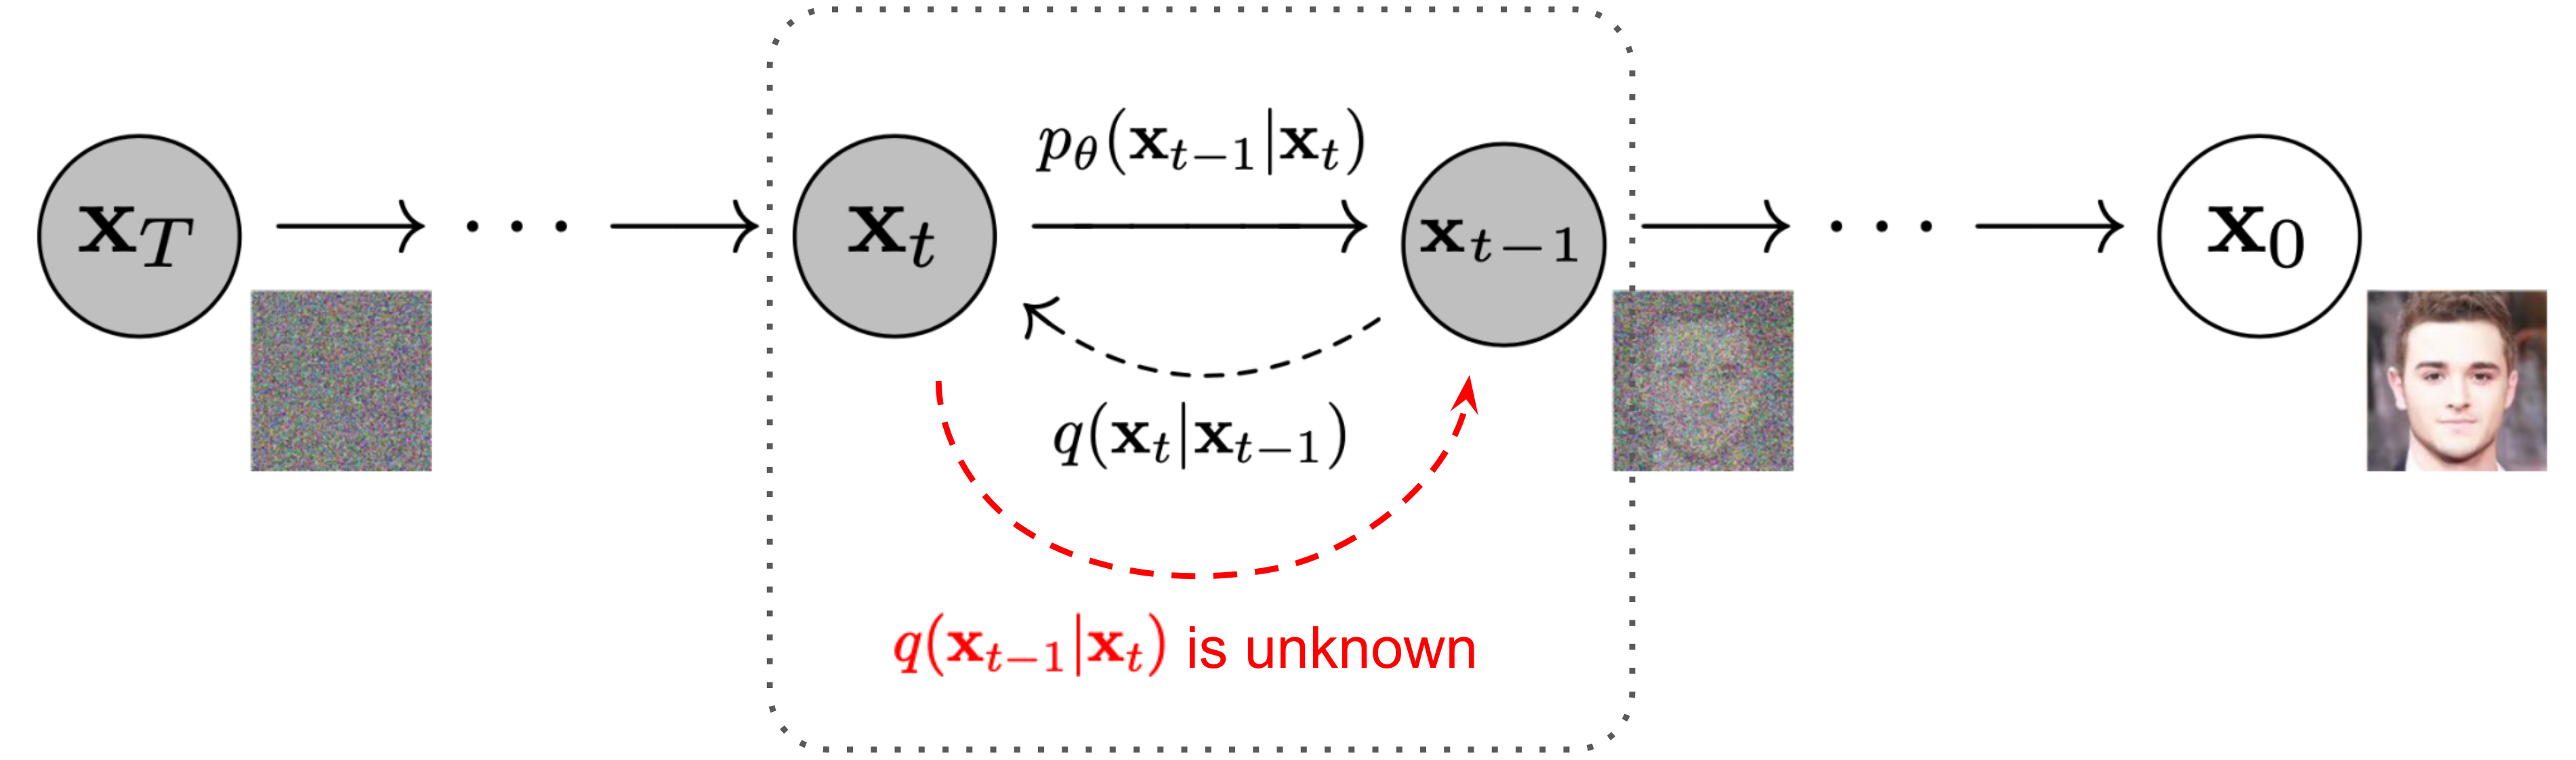
\includegraphics[width=0.8\linewidth]{figs/DDPM}
	\end{figure}
	\vspace{-0.3cm}
	\begin{block}{Reverse gaussian diffusion process}
		\vspace{-0.6cm}
		\begin{align*}
			q(\bx_{t-1}|\bx_{t}) &= \frac{q(\bx_{t}|\bx_{t-1}) {\color{violet}q(\bx_{t-1})}}{{\color{violet}q(\bx_{t})}} \\
			q(\bx_{t-1}|\bx_{t}, {\color{olive}\bx_0}) &= \frac{q(\bx_{t}|\bx_{t-1}, {\color{olive}\bx_0}) q(\bx_{t-1} | {\color{olive}\bx_0}) }{q(\bx_{t}| {\color{olive}\bx_0})} = \cN(\tilde{\bmu}_t(\bx_t, \bx_0), \tilde{\beta}_t \bI)
		\end{align*}
		\vspace{-0.6cm}
		\begin{itemize}
			\item ${\color{violet}q(\bx_{t-1})}$, ${\color{violet}q(\bx_{t})}$ are intractable.
			\item If $\beta_t$ is small enough, $q(\bx_{t-1}|\bx_{t})$ will be Gaussian (Feller, 1949).
			\item $q(\bx_{t-1} | \bx_t, \bx_0)$ defines how to denoise a noisy image $\bx_t$ with access to the completely denoised image $\bx_0$.
		\end{itemize}
	\end{block}
	\myfootnotewithlink{https://lilianweng.github.io/posts/2021-07-11-diffusion-models/}{Weng L. What are Diffusion Models?, blog post, 2021}
\end{frame}
%=======
\begin{frame}{Recap of previous lecture}
	Let define the reverse process
	\vspace{-0.2cm}
	\[
		q(\bx_{t-1}|\bx_{t}) \approx p(\bx_{t - 1} | \bx_t, \btheta) = \cN \bigl(\bx_{t - 1} | \bmu_{\btheta}(\bx_t, t), \bsigma_{\btheta}^2(\bx_t, t)\bigr)
	\]
	\begin{minipage}{0.5\linewidth}
		\begin{block}{Forward process}
			\begin{enumerate}
				\item $\bx_0 = \bx \sim \pi(\bx)$;
				\item $\bx_t = \sqrt{1 - \beta_t} \cdot \bx_{t - 1} + \sqrt{\beta_t} \cdot \bepsilon$, where $\bepsilon \sim \cN(0, \bI)$, $t \geq 1$;
				\item $\bx_T \sim p_{\infty}(\bx) = \cN(0, \bI)$.
			\end{enumerate}
		\end{block}
	\end{minipage}%
	\begin{minipage}{0.5\linewidth}
		\begin{block}{Reverse process}
			\begin{enumerate}
				\item $\bx_T \sim p_{\infty}(\bx) = \cN(0, \bI)$;
				\item $\bx_{t - 1} = \bsigma_{\btheta}(\bx_t, t) \cdot \bepsilon + \bmu_{\btheta}(\bx_t, t)$;
				\item $\bx_0 = \bx \sim \pi(\bx)$;
			\end{enumerate}
		\end{block}
	\end{minipage}
	\begin{block}{Gaussian diffusion model as VAE}
		\vspace{-0.3cm}
		\begin{figure}
			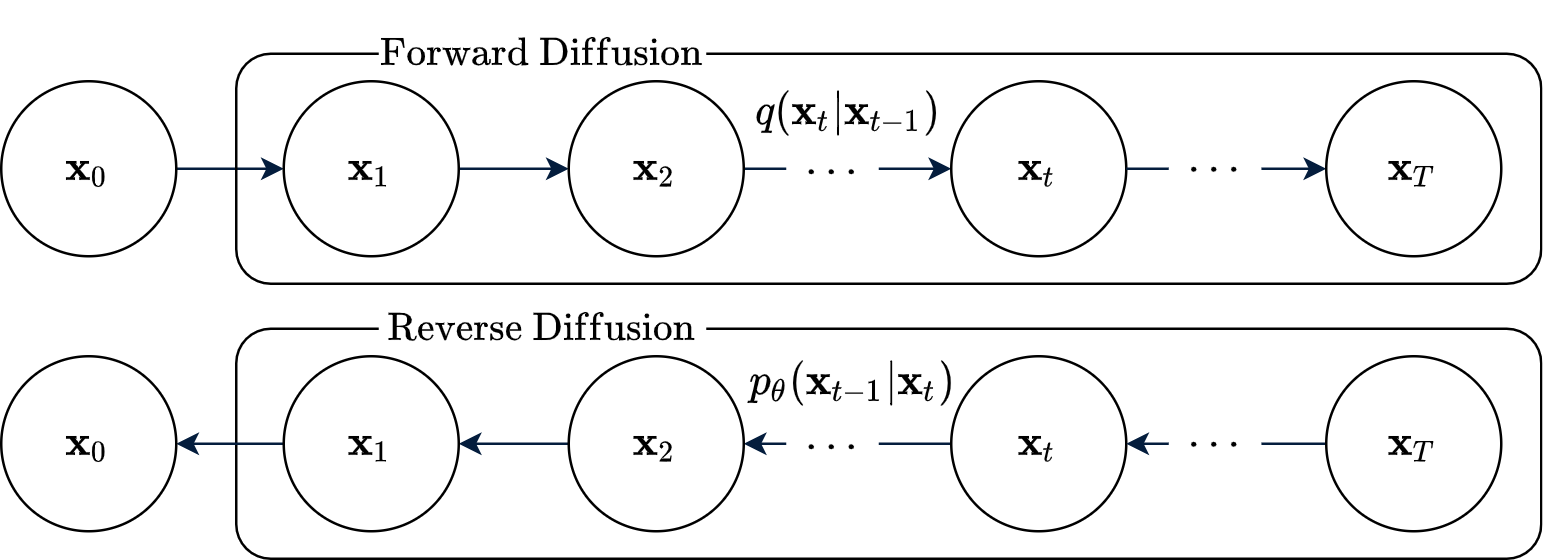
\includegraphics[width=0.65\linewidth]{figs/diffusion_pgm}
		\end{figure}
	\end{block}
	\myfootnotewithlink{https://lilianweng.github.io/posts/2021-07-11-diffusion-models/}{Weng L. What are Diffusion Models?, blog post, 2021}
\end{frame}
%=======
\begin{frame}{Recap of previous lecture}
	\begin{itemize}
		\item $\bz = (\bx_1, \dots, \bx_T)$ is a latent variable.
		\item Variational posterior distribution
		\vspace{-0.2cm}
		\[
			q(\bz | \bx) = q(\bx_1, \dots, \bx_T | \bx_0) = \prod_{t = 1}^T q(\bx_t | \bx_{t - 1}).
		\]
		\vspace{-0.3cm}
		\item Generative distribution and prior
		\vspace{-0.2cm}
		\[
			p(\bx | \bz, \btheta) = p(\bx_0 | \bx_1, \btheta); \quad 
			p(\bz | \btheta) = \prod_{t=2}^T p(\bx_{t - 1} | \bx_t, \btheta) \cdot p(\bx_T)
		\]
	\end{itemize}
	\vspace{-0.2cm}
	\begin{block}{ELBO}
		\vspace{-0.2cm}
		\[
			\log p(\bx | \btheta) \geq \bbE_{q({\color{teal}\bz} | \bx)} \log \frac{p(\bx, {\color{teal}\bz} | \btheta)}{q({\color{teal}\bz} | \bx)} = \cL(q, \btheta) \rightarrow \max_{q, \btheta}
		\]
		\vspace{-0.5cm}
		\begin{multline*}
			\cL(q, \btheta) =  {\color{olive}\bbE_{q(\bx_1 | \bx_0)} \log p(\bx_0 | \bx_1, \btheta)} - {\color{violet}KL\bigl(q(\bx_T | \bx_0) || p(\bx_T)\bigr)} - \\
			- \sum_{t=2}^T  \underbrace{ \bbE_{q(\bx_t | \bx_0)}KL \bigl(q(\bx_{t-1} | \bx_t, \bx_0) || p(\bx_{t - 1} | \bx_t, \btheta )\bigr)}_{\cL_t}
		\end{multline*}
	\end{block}
	\myfootnotewithlink{https://ayandas.me/blog-tut/2021/12/04/diffusion-prob-models.html}{Das A. An introduction to Diffusion Probabilistic Models, blog post, 2021}
\end{frame}
%=======
\begin{frame}{Outline}
	\tableofcontents
\end{frame}
%=======
\section{Denoising Diffusion Probabilistic Model (DDPM)}
%=======
\subsection{Reparametrization of gaussian diffusion model}
%=======
\begin{frame}{Reparametrization of DDPM}
	\[
		\cL_t = \bbE_{q(\bx_t | \bx_0)} KL \bigl(q(\bx_{t-1} | \bx_t, \bx_0) || p(\bx_{t - 1} | \bx_t, \btheta )\bigr)
	\]
	$\cL_t$ is the mean of KL between two normal distributions:
	\begin{align*}
		q(\bx_{t-1} | \bx_t, \bx_0) &= \cN(\bx_{t-1} | \tilde{\bmu}_t(\bx_t, \bx_0), \tilde{\beta}_t \bI), \\
		p(\bx_{t - 1} | \bx_t, \btheta) &= \cN \bigl(\bx_{t - 1} | \bmu_{\btheta}(\bx_t, t), {\color{violet}\bsigma_{\btheta}^2(\bx_t, t)}\bigr)
	\end{align*}
	Here
	\begin{align*}
		\tilde{\bmu}_t(\bx_t, \bx_0) &= \frac{\sqrt{\alpha_t}(1 - \bar{\alpha}_{t-1})}{1 - \bar{\alpha}_t} \bx_t + \frac{\sqrt{\bar{\alpha}_{t-1}}(1 - \alpha_t)}{1 - \bar{\alpha}_t} \bx_0; \\
		\tilde{\beta}_t &= \frac{(1 - \alpha_t)(1 - \bar{\alpha}_{t-1})}{1 - \bar{\alpha}_t} = \text{const}.
	\end{align*}
	Let assume
	\[
		{\color{violet}\bsigma_{\btheta}^2(\bx_t, t) = \tilde{\beta}_t \bI} \quad \Rightarrow \quad p(\bx_{t - 1} | \bx_t, \btheta) = \cN \bigl(\bx_{t - 1} | \bmu_{\btheta}(\bx_t, t), {\color{violet}\tilde{\beta}_t \bI} \bigr).
	\]
	\myfootnotewithlink{https://arxiv.org/abs/2006.11239}{Ho J. Denoising Diffusion Probabilistic Models, 2020}
\end{frame}
%=======
\begin{frame}{Reparametrization of DDPM}
	\vspace{-0.5cm}
	\begin{align*}
		q(\bx_{t-1} | \bx_t, \bx_0) &= \cN(\bx_{t-1} | \tilde{\bmu}_t(\bx_t, \bx_0), \tilde{\beta}_t \bI); \\
		p(\bx_{t - 1} | \bx_t, \btheta) &= \cN (\bx_{t - 1} | \bmu_{\btheta}(\bx_t, t), \tilde{\beta}_t \bI ).
	\end{align*}
	Use the formula for KL between two normal distributions:
	\begin{align*}
		\cL_t &= \bbE_{q(\bx_t | \bx_0)} KL\Bigl(\cN\bigl(\tilde{\bmu}_t(\bx_t, \bx_0), \tilde{\beta}_t \bI \bigr) || \cN\bigl(\bmu_{\btheta}(\bx_t, t), \tilde{\beta}_t \bI\bigr)\Bigr) \\ 
		&= \bbE_{q(\bx_t | \bx_0)} \left[\frac{1}{2\tilde{\beta}_t} \bigl\| \tilde{\bmu}_t(\bx_t, \bx_0) - \bmu_{\btheta}(\bx_t, t) \bigr\|^2  \right]
	\end{align*}
	\vspace{-0.2cm}
	\[
		\bx_t = \sqrt{\bar{\alpha}_t} \bx_0 + \sqrt{1 - \bar{\alpha}_t} \bepsilon \quad \Rightarrow \quad {\color{olive} \bx_0} = \frac{\bx_t -  \sqrt{1 - \bar{\alpha}_t} \bepsilon}{\sqrt{\bar{\alpha}_t}}
	\]
	\vspace{-0.2cm}
	\begin{align*}
		\tilde{\bmu}_t(\bx_t, \bx_0) &= \frac{\sqrt{\alpha_t}(1 - \bar{\alpha}_{t-1})}{1 - \bar{\alpha}_t} \bx_t + \frac{\sqrt{\bar{\alpha}_{t-1}}(1 - \alpha_t)}{1 - \bar{\alpha}_t} {\color{olive} \bx_0} \\
		&= \frac{1}{\sqrt{\alpha_t}} \bx_t - \frac{1 - \alpha_t}{\sqrt{\alpha_t (1 - \bar{\alpha}_t)}} \bepsilon
	\end{align*}
	\myfootnotewithlink{https://arxiv.org/abs/2006.11239}{Ho J. Denoising Diffusion Probabilistic Models, 2020}
	\end{frame}
%=======
\begin{frame}{Reparametrization of DDPM}
	\vspace{-0.3cm}
	\[
		\cL_t = \bbE_{\color{violet}q(\bx_t | \bx_0)} \left[ {\color{olive}\frac{1}{2\tilde{\beta}_t}} \bigl\| \tilde{\bmu}_t(\bx_t, \bx_0) - \bmu_{\btheta}(\bx_t, t) \bigr\|^2  \right]
	\]
	\vspace{-0.3cm}
	\begin{block}{Reparametrization}
		\vspace{-0.7cm}
		\begin{align*}
			\tilde{\bmu}_t(\bx_t, \bx_0) &= \frac{1}{\sqrt{\alpha_t}} \bx_t - \frac{1 - \alpha_t}{\sqrt{\alpha_t (1 - \bar{\alpha}_t)}} \bepsilon \\
			\bmu_{\btheta}(\bx_t, t) &= \frac{1}{\sqrt{\alpha_t}} \bx_t - {\color{teal}\frac{1 - \alpha_t}{\sqrt{\alpha_t (1 - \bar{\alpha}_t)}}} \bepsilon_{\btheta}(\bx_t, t)
		\end{align*}
		\vspace{-0.7cm}
	\end{block}
		\vspace{-0.5cm}
		\begin{align*}
			\cL_t &=  \bbE_{\color{violet} \bepsilon \sim \cN(0, \bI)} \left[ \frac{{\color{teal}(1 - \alpha_t)^2}}{{\color{olive}2\tilde{\beta}_t} {\color{teal} \alpha_t (1 - \bar{\alpha}_t)}} \bigl\| \bepsilon - \bepsilon_{\btheta}({\color{violet}\bx_t}, t) \bigr\|^2 \right] \\
			& =	 \bbE_{\color{violet}\bepsilon \sim \cN(0, \bI)} \left[ \frac{(1 - \alpha_t)^2}{2\tilde{\beta}_t \alpha_t (1 - \bar{\alpha}_t)} \Bigl\| \bepsilon - \bepsilon_{\btheta}\bigl( {\color{violet}\sqrt{\bar{\alpha}_t} \bx_0 + \sqrt{1 - \bar{\alpha}_t} \bepsilon}, t\bigr) \Bigr\|^2 \right]
		\end{align*}
		At each step of reverse diffusion process we try to predict the noise~$\bepsilon$ that we used in the forward diffusion process!
	\myfootnotewithlink{https://arxiv.org/abs/2006.11239}{Ho J. Denoising Diffusion Probabilistic Models, 2020}
	\end{frame}
%=======
\begin{frame}{Reparametrization of DDPM}
	\begin{multline*}
		\cL(q, \btheta) =  {\color{olive}\bbE_{q(\bx_1 | \bx_0)} \log p(\bx_0 | \bx_1, \btheta)} - {\color{violet}KL\bigl(q(\bx_T | \bx_0) || p(\bx_T)\bigr)} - \\
		- \sum_{t=2}^T \underbrace{ \bbE_{q(\bx_t | \bx_0)} KL \bigl(q(\bx_{t-1} | \bx_t, \bx_0) || p(\bx_{t - 1} | \bx_t, \btheta )\bigr)}_{\cL_t}
	\end{multline*}
	\vspace{-0.3cm}
	\[
		\cL_t  = \bbE_{\bepsilon \sim \cN(0, \bI)} \left[ \frac{(1 - \alpha_t)^2}{2\tilde{\beta}_t \alpha_t (1 - \bar{\alpha}_t)} \Bigl\| \bepsilon - \bepsilon_{\btheta}\bigl( \sqrt{\bar{\alpha}_t} \bx_0 + \sqrt{1 - \bar{\alpha}_t} \bepsilon, t\bigr) \Bigr\|^2 \right]
	\]
	\begin{block}{Simplified objective}
		\[
			 \cL_{\text{simple}} = \bbE_{t \sim U[2, T]} \bbE_{\bepsilon \sim \cN(0, \bI)} \Bigl\| \bepsilon - \bepsilon_{\btheta}\bigl( \sqrt{\bar{\alpha}_t} \bx_0 + \sqrt{1 - \bar{\alpha}_t} \bepsilon, t\bigr) \Bigr\|^2 
		\]
	\end{block}
	\myfootnotewithlink{https://arxiv.org/abs/2006.11239}{Ho J. Denoising Diffusion Probabilistic Models, 2020}
	\end{frame}
%=======
\subsection{Overview of DDPM}
%=======
\begin{frame}{Denoising diffusion probabilistic model (DDPM)}
	\begin{block}{DDPM is a VAE model}
		\begin{itemize}
			\item Encoder is a fixed Gaussian Markov chain $q(\bx_1, \dots, \bx_T | \bx_0)$.
			\item Latent variable is a hierarchical (in each step the dim. of the latent equals to the dim of the input).
			\item Decoder is a simple Gaussian model $p(\bx_0 | \bx_1, \btheta)$.
			\item Prior distribution is given by parametric Gaussian Makov chain $p(\bx_{t-1} | \bx_t, \btheta)$.
		\end{itemize}
	\end{block}
	\begin{minipage}{0.5\linewidth}
		\begin{block}{Forward process}
			\begin{enumerate}
				\item $\bx_0 = \bx \sim \pi(\bx)$;
				\item $\bx_t = \sqrt{1 - \beta_t} \cdot \bx_{t - 1} + \sqrt{\beta_t} \cdot \bepsilon$, where $\bepsilon \sim \cN(0, \bI)$, $t \geq 1$;
				\item $\bx_T \sim p_{\infty}(\bx) = \cN(0, \bI)$.
			\end{enumerate}
		\end{block}
	\end{minipage}%
	\begin{minipage}{0.5\linewidth}
		\begin{block}{Reverse process}
			\begin{enumerate}
				\item $\bx_T \sim p_{\infty}(\bx) = \cN(0, \bI)$;
				\item $\bx_{t - 1} = \bsigma_{\btheta}(\bx_t, t) \cdot \bepsilon + \bmu_{\btheta}(\bx_t, t)$;
				\item $\bx_0 = \bx \sim \pi(\bx)$;
			\end{enumerate}
		\end{block}
	\end{minipage}
\end{frame}
%=======
\begin{frame}{Denoising diffusion probabilistic model (DDPM)}
	\begin{block}{Training}
		\begin{enumerate}
			\item Get the sample $\bx_0 \sim \pi(\bx)$.
			\item Sample timestamp $t \sim U[1, T]$ and the noise $\bepsilon \sim \cN(0, \bI)$.
			\item Get noisy image $\bx_t = \sqrt{\bar{\alpha}_t} \bx_0 + \sqrt{1 - \bar{\alpha}_t} \bepsilon$.
			\item Compute loss $ \cL_{\text{simple}} = \| \bepsilon - \bepsilon_{\btheta}(\bx_t , t) \|^2 $.
		\end{enumerate}
	\end{block}
	\begin{block}{Sampling}
		\begin{enumerate}
			\item Sample $\bx_T \sim \cN(0, \bI)$.
			\item Compute mean of $p(\bx_{t-1} | \bx_t, \btheta) = \cN(\bmu_{\btheta}(\bx_t, t), \tilde{\beta}_t \bI)$:
			\[
				\bmu_{\btheta}(\bx_t, t) = \frac{1}{\sqrt{\alpha_t}} \bx_t - \frac{1 - \alpha_t}{\sqrt{\alpha_t (1 - \bar{\alpha}_t)}} \bepsilon_{\btheta}(\bx_t, t)
			\]
			\vspace{-0.3cm}
			\item Get denoised image $\bx_{t - 1} = \bmu_{\btheta}(\bx_t, t) +  \sqrt{\tilde{\beta}_t} \cdot \bepsilon$, where $\bepsilon \sim \cN(0, \bI)$.
		\end{enumerate}
	\end{block}
	\myfootnotewithlink{https://arxiv.org/abs/2006.11239}{Ho J. Denoising Diffusion Probabilistic Models, 2020}
\end{frame}
%=======
\begin{frame}{Denoising diffusion probabilistic model (DDPM)}
	\begin{block}{Samples}
		\begin{figure}
			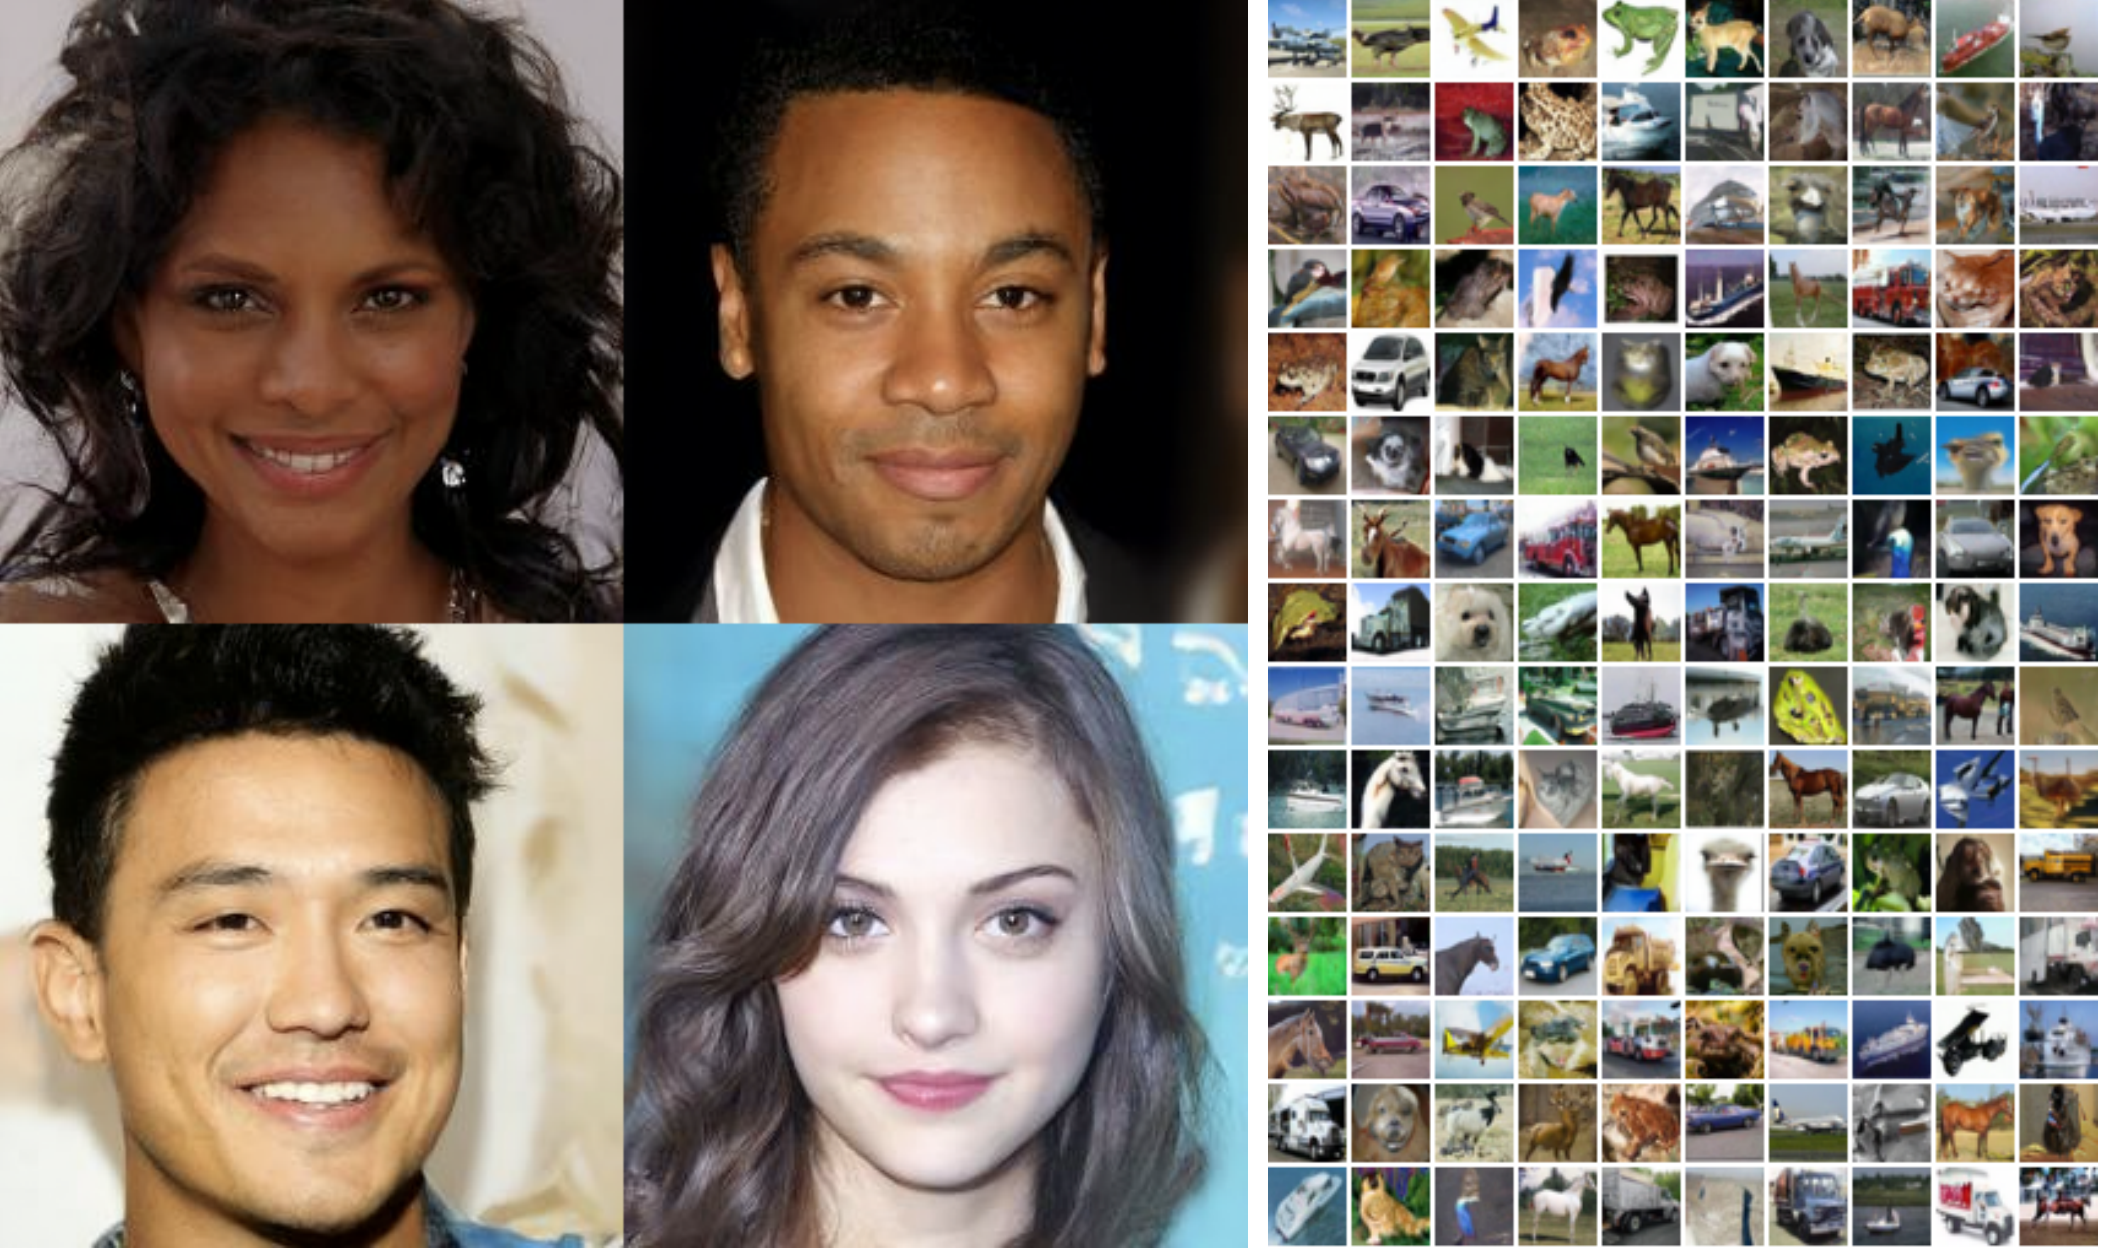
\includegraphics[width=\linewidth]{figs/ddpm_samples}
		\end{figure}
	\end{block}
	\myfootnotewithlink{https://arxiv.org/abs/2006.11239}{Ho J. Denoising Diffusion Probabilistic Models, 2020}
\end{frame}
%=======
\section{Langevin dynamic}
%=======
\begin{frame}{Langevin dynamic}
	\vspace{-0.4cm}
	\begin{block}{Statement}
		Let $\bx_0$ be a random vector. Then samples from the following dynamics
		\vspace{-0.3cm}
		\[
			\bx_{t + 1} = \bx_t + \eta \frac{1}{2} \nabla_{\bx_t} \log p(\bx_t | \btheta) + \sqrt{\eta} \cdot \bepsilon, \quad \bepsilon \sim \cN(0, \bI).
		\]
		will come from $p(\bx | \btheta)$ under mild regularity conditions for small enough $\eta$ and large enough $t$.
	\end{block}
	\begin{minipage}{0.55\linewidth}
		\begin{itemize}
			\item Here we assume that we already have some generative model $p(\bx | \btheta)$.
			\item The density $p(\bx | \btheta)$ is a \textbf{stationary} distribution for this SDE. \\
			\item What do we get if $\bepsilon = \boldsymbol{0}$?
		\end{itemize}
	\end{minipage}%
	\begin{minipage}{0.4\linewidth}
		\begin{figure}
			\centering
			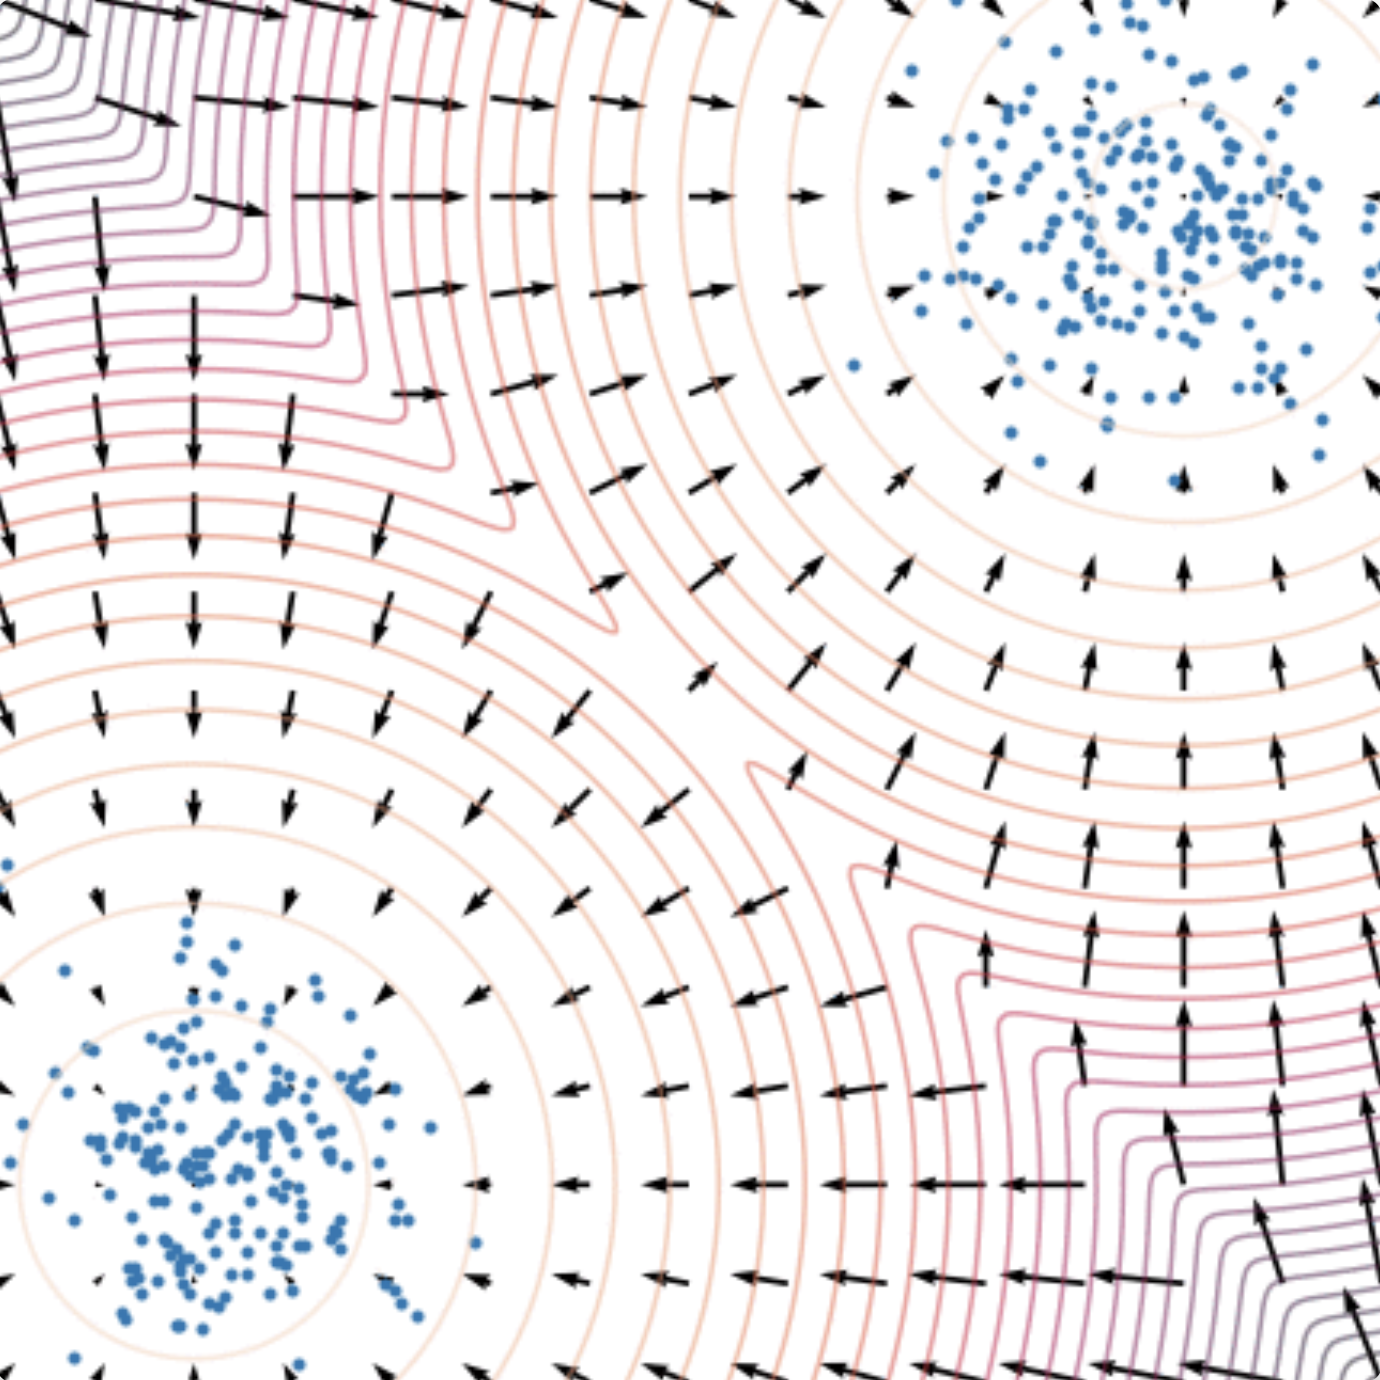
\includegraphics[width=0.9\linewidth]{figs/langevin_dynamic}
		\end{figure}
	\end{minipage}
	\myfootnotewithlink{https://yang-song.github.io/blog/2021/score/}{Song Y. Generative Modeling by Estimating Gradients of the Data Distribution, blog post, 2021} 
	\end{frame}
%=======
\begin{frame}{Energy-based models}
	\begin{itemize}
		\item We could sample from the model using Langevin dynamics if we have $\nabla_{\bx}\log p(\bx| \btheta)$.
		\item Where is it helpful?
	\end{itemize}
	\begin{block}{Unnormalized density}
		\vspace{-0.2cm}
		\[
			p(\bx | \btheta) = \frac{\hat{p}(\bx | \btheta)}{Z_{\btheta}}, \quad \text{where } Z_{\btheta} = \int \hat{p}(\bx | \btheta) d \bx
		\]
		\begin{itemize}
			\item $\hat{p}(\bx | \btheta)$ is any non-negative function. \\
			\item If we use the reparametrization $\hat{p}(\bx | \btheta) = \exp(-f_{\btheta}(\bx))$, we remove the non-negativite constraint.
		\end{itemize}
		\[
			\nabla_{\bx} \log p(\bx | \btheta) = \nabla_{\bx} \log \hat{p}(\bx | \btheta) - \nabla_{\bx} \log Z_{\btheta} = \nabla_{\bx} \log \hat{p}(\bx | \btheta)
		\]
		The gradient of the normalized density equals to the gradient of the unnormalized density.
	\end{block}
\end{frame}
%=======
\begin{frame}{Score matching}
	We could sample from the model using Langevin dynamics if we have $\nabla_{\bx}\log p(\bx| \btheta)$.
	\begin{block}{Fisher divergence}
		\vspace{-0.3cm}
		\[
		D_F(\pi, p) = \frac{1}{2}\bbE_{\pi}\bigl\| \nabla_{\bx}\log p(\bx| \btheta) - \nabla_\bx \log \pi(\bx) \bigr\|^2_2 \rightarrow \min_{\btheta}
		\]
		\vspace{-0.5cm}
	\end{block}
	Let introduce \textbf{score function} $\bs_{\btheta}(\bx) = \nabla_{\bx}\log p(\bx| \btheta)$. 
	\vspace{-0.2cm}
	\begin{figure}
		\centering
		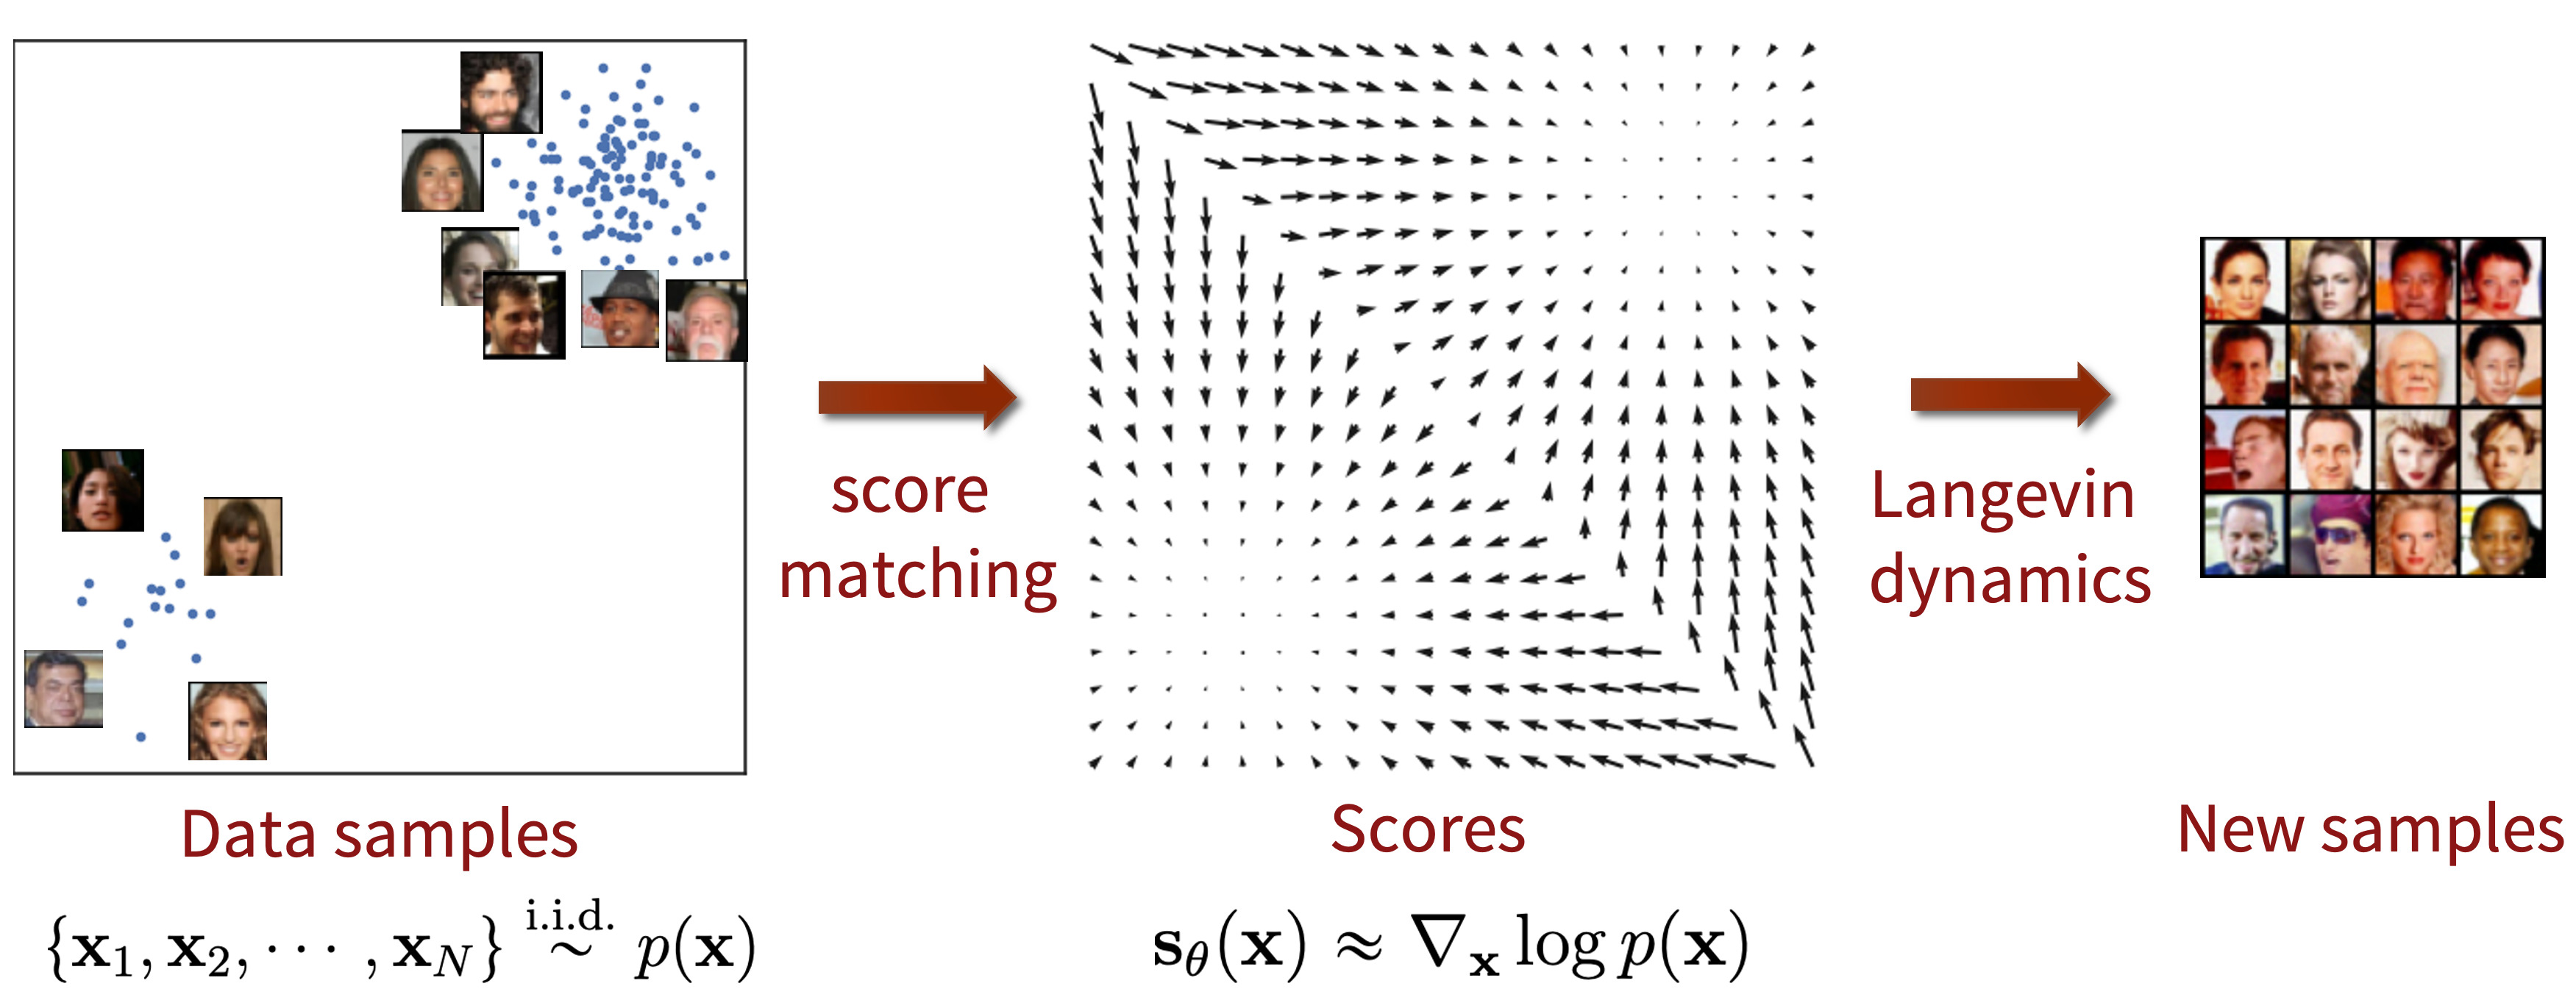
\includegraphics[width=0.75\linewidth]{figs/smld}
	\end{figure}
	\vspace{-0.3cm} 
	\textbf{Problem:} we do not know $\nabla_\bx \log \pi(\bx)$.
	\myfootnotewithlink{https://yang-song.github.io/blog/2021/score/}{Song Y. Generative Modeling by Estimating Gradients of the Data Distribution, blog post, 2021}
\end{frame}
%=======
\begin{frame}{Summary}
	\begin{itemize}
		\item DDPM is a VAE model with hierarchical latent variables.
		\vfill
		\item At each step DDPM predicts the noise that was used in the forward diffusion process.
		\vfill
		\item DDPM is really slow, because we have to apply the model $T$ times.
		\vfill
		\item Langevin dynamics allows to sample from the generative model using the gradient of the log-likelihood.	
		\vfill
		\item Score matching proposes to minimize Fisher divergence to get the score function.
	\end{itemize}
\end{frame}
\end{document} 